\section{Evaluation}
\label{sec\:eval}
To evaluate the effectiveness of \sysname{}, we design and conduct two case study scenarios representing realistic deployment use cases. These scenarios allow us to examine \sysname{}\textquotesingle s capabilities under both targeted and open-ended conditions, and to compare its behavior against state-of-the-art detection methods.

\begin{enumerate}
\item \textit{Configuration Update Verification}: This scenario focuses on verifying the correctness of incremental configuration changes. \sysname{} is applied to recent updates in campus network configurations, each consisting of a set of added or modified lines. These updates include both correct and faulty changes, grounded in real network deployment logs. The objective is to determine whether \sysname{} can accurately detect misconfigurations introduced specifically by the updates, without scanning the full configuration.

\item \textit{Comprehensive Configuration Verification}: In this broader scenario, \sysname{} is applied to entire configuration snapshots drawn from (A) a medium-scale campus network using Aruba devices and (B) a large-scale campus network using Cisco devices. Unlike the previous task, no update information is provided. Instead, \sysname{} must examine full configurations to surface misconfigurations. We evaluate both \textit{targeted detection}—focusing on known issue types (\eg, VLAN assignment errors, port misalignments), using only configurations from Campus A where such issues are known to occur—and \textit{non-targeted detection}, where the goal is to identify latent issues in a free-form scan across both Campus A and Campus B.

\end{enumerate}

\aaron{The two parts of the evaluation feel disconnected, and the flow could be improved. In particular, 6.2 presents some \sysname{} accuracy results followed by a comparison with prior work, then 6.3 presents more \sysname{} accuracy results on completely different configurations with no comparison with prior work. It feels odd to have comparison with prior tools between the accuracy results, and it is not clear why different configs are used for the different parts---I realize that the evaluation was conducted this way, but there needs to be an explanation provided. Also, the targeted analysis for Campus A in 6.3 feels out of place, because there is no targeted analysis for Campus B, and section 6.1 already did targeted analysis. Similarly, false positives and comparisons between LLMs are discussed in both 6.3 and 6.4, which seems redundant.

I propose that we restructure the evaluation to focus on the following questions (in subsections in order):
\begin{enumerate}
\item Can \sysname{} detect known misconfigurations? -- this is a simple starting point; includes \sysname{} results for synthetic misconfigs introduced in Internet2 (part of Section 6.2, Table 2, part of Table 3, and Table 4) and results for known VLAN issue in campus A (part of Section 6.3, top row in Table 5)
\item Can \sysname{} accurately identify new issues? -- includes non-targeted results for campus A (part of Section 6.3 and part of Table 5) and non-targeted results for campus B (part of Section 6.3, Table 6, and part of Section 6.4)
\item What context do LLMs request? -- includes requested contexts for synthetic misconfigs (part of Table 2) and requested contexts for non-targeted campus A and B (Table 7, Table 8, Figure 6, and part of Section 6.4)
\item How does \sysname{} compare to existing tools? -- includes Batfish, Diffy, Ciri, and FFP results for synthetic misconfigs (part of Table 3 and part of Section 6.2) and non-targeted campus A and B (to be gathered?)
\end{enumerate}
}


We now describe the setup used to support these evaluation scenarios and provide detailed findings in subsequent sections.

\subsection{Evaluation Setup}

\mypara{Context Extraction Hardware:}
%\textit{System Information}: GNU/Linux Red Hat Enterprise Linux release 8.8 (Ootpa) \aaron{I don't think OS matters};
%\textit{CPU Specifications}: Architecture: x86\_64; CPU(s): 32 (2 threads/core, 16 cores/socket, 1 socket); Model: AMD EPYC 7302P 16-Core Processor; Max MHz: 3000.000; L3 cache: 16384K; NUMA node0 CPU(s): 0--31.
The system we use for context extraction has a single AMD EPYC 7302P (3GHz, 16-Core/32-Thread, 128MB L3 cache) processor and \aaron{???}GB of memory.
We do not use GPU acceleration, because \sysname{}'s context extraction and orchestration logic is CPU-parallelizable and does not significantly benefit from GPU throughput.

\mypara{Querying LLMs:}
We evaluate \sysname{} using GPT-4o~~\cite{openai_gpt4o}---OpenAI's latest model optimized for complex reasoning and long-context tasks (Context window: 128,000 tokens; Max output: 4,096 tokens; Training cutoff: October 2023)---and DeepSeek-V3 (DS)~~\cite{deepseekai2024deepseekv3technicalreport}---DeepSeek-AI's open-source transformer suited for structured code and configuration analysis (Context window: 128,000 tokens; Max output: 8,000 tokens; Training cutoff: July 2024). We use OpenAI's and DeepSeeks's Chat Completions APIs. \aaron{Does it matter which API we use?} Each interaction includes a structured conversation history to simulate persistent reasoning. \aaron{Move the details about prompts to the relevant subsections fo the evaluation?} Prompts are crafted based on the scenario type: in the targeted setting, the prompts focus on verifying specific change lines or known risks; in the non-targeted setting, the model is instructed to surface any misconfigurations based on general policy correctness and best practices. Figures~\ref{fig:initial_prompt} and~\ref{fig:feedback_and_response} provide representative examples.

\mypara{Model Usage by Scenario:} \aaron{This is mostly redundant with the opening of the introduction}
\begin{itemize}
\item \textbf{Configuration Update Verification.} \textcolor{red}{Only one model (GPT-4o)} is used for this task. This setting is used to test whether a widely available, general-purpose LLM is sufficient for accurately identifying misconfigurations in well-scoped scenarios. Since the detection task is clearly defined and limited to specific configuration updates, a single model is adequate for evaluating feasibility.

\item \textbf{Comprehensive Configuration Verification.} \textcolor{red}{Both GPT-4o and DeepSeek-V3} are used. This setup is intentionally open-ended, allowing us to evaluate whether model choice affects misconfiguration discovery. Additionally, because this task relies on \sysname{}'s guided interactive prompting mechanism, we can observe whether different models exhibit divergent patterns in their context requests, reasoning steps, or detection results. This comparison helps us understand the sensitivity of the \sysname{} pipeline to the underlying language model.
\end{itemize}


\aaron{TODO: Provide an overview of the configurations used from Internet2, Campus A, and Campus B---number of devices, vendors, device roles, config lengths. A table is an effective/concise way to present this.}


\subsection{Case Study 1: Configuration Update Verification}
We first test \sysname{}'s effectiveness in handling configuration updates, aiming to verify its ability to capture various types of misconfigurations and accurately assess detection performance in a controlled environment. \aaron{Considering this subsection of the evaluation to be about updates (and Section 6.3 to not be about updates) seems like a mischaracterization. The key difference between the \sysname{} results in this subsection and Section 6.3 is that the synthetic errors introduced into Internet2 are known misconfigurations, whereas Section 6.3 is mostly about finding new issues (except for the targeted misconfigs in campus A). It seems more accurate to differentiate between evaluating \sysname{}'s ability to detect known misconfigs versus \sysname{}'s accuracy in identifying new issues--as outlined in my comment at the beginning of the Evaluation section.}
Router misconfigurations are broadly categorized into three types:
\begin{itemize}
    \item \textit{Syntax errors} occur when the configuration does not adhere to the expected format or structure---\eg, a missing bracket or misused keyword in a BGP routing policy.
    \item \textit{Range violations} involve parameter values that fall outside the acceptable range---\eg, an MTU value that exceeds the maximum allowed for a specific interface type.
    \item \textit{Dependency/conflict (D/C) issues} arise when different configuration lines are incompatible or contradict each other---\eg, a firewall rule might block traffic that another policy explicitly permits. \aaron{Could we divide this category in half, such that we have 4 types of each error? E.g., could we separate into dependency and consistency?}
\end{itemize}

\aaron{Citing some related work---e.g., misconfigs uncovered using existing tools---as inspiration for these categories could strengthen this part of the evaluation.}

% \begin{table}[tb]
% \centering
% \resizebox{\columnwidth}{!}{
% \begin{tabular}{|l|l|l|l|}
% \hline
% \textbf{Type} & \textbf{Description} & \textbf{Misconfig} & \textbf{Requested Context}\\ \hline

% \multirow{4}{*}{\textbf{Syntax}} 
% & Missing brace &...interfaces: \{\textcolor{red}{"<ge-*"}: & None\\ \cline{2-4}
% & Invalid keyword & ...mtu: \textcolor{red}{"True"}   & \( N(P) \), \( R(P) \)\\ \cline{2-4}
% & Incorrect hierarchy & ...host-name: \textcolor{red}{"\{rtsw.alba-re1\}"}  & \( N(P) \)\\ \cline{2-4}
% & Invalid IP address & ...neighbor: \textcolor{red}{192.168.253.1.1}" & \( N(P) \), \( R(P) \)\\ \hline

% \multirow{4}{*}{\textbf{Range}}  
% & Invalid MTU & ...mtu: \textcolor{red}{"10000"}  & \( N(P) \), \( R(P) \)\\ \cline{2-4}
% & Invalid VLAN ID & ...vlan-id: \textcolor{red}{"5000"}  & \( N(P) \), \( R(P) \), \( R(N(P)) \) \\ \cline{2-4}
% & Invalid AS & ...autonomous-system: \textcolor{red}{70000} & \( N(P) \), \( R(P) \) \\ \cline{2-4}
% & Invalid prefix limit & ...maximum: \textcolor{red}{"200000"} & \( N(P) \), \( R(P) \)  \\ \hline

% \multirow{8}{*}{\textbf{D/C}}  
% & Non-existent group & ... apply-groups: \textcolor{red}{"L2-LSP-ATTRIBUTES”} & \( N(P) \), \( R(P) \), \( R(N(P)) \) \\ \cline{2-4}
% & Policy Conflict & ...community \textcolor{red}{add I2CLOUD-EXTENDED-TARGET}  & \( N(P) \), \( R(P) \), \( R(N(P)) \) \\ \cline{2-4}
% & Non-existent filter & ...input-list: \textcolor{red}{"uplink"} & \( N(P) \), \( R(P) \)  \\ \cline{2-4}
% & Non-existent policy & ...export: \textcolor{red}{"OESS-400-300-LOOP} & \( R(P) \)  \\ \cline{2-4}
% & Incorrect Filter Usage & ...family mpls: filter:input-list:\textcolor{red}{"v6filter"} & \( R(P), S(P) \)  \\ \cline{2-4}
% & Disabled Sampling & ...family inet6: \textcolor{red}{SAMPLING MISSING/DISABLED}& \( R(P), N(P) \)  \\ \cline{2-4}
% & VRF Target Conflict & ...vrf-target target:11537:\textcolor{red}{"313001"}& \( S(P) \)  \\ \cline{2-4}
% & Abnormal Small MTU & ...family iso: mtu: \textcolor{red}{"1497"}& \( R(P), S(P) \)  \\ \hline
% \end{tabular}}
% \caption{Erroneous Configuration Updates Introduced and LLM Requested Context for \sysname{}. \aaron{What is a "Policy conflict"? What is "Incorrect Filter Usage"? What is sampling disabled for? What is "VRF Target Conflict"?} \aaron{Are the errors introduced in the "groups" section at the top of the configs? (Groups are a unique feature of Juniper configs which existing tools may be ill-equipped to reason about, making existing tools look worse than they actually are.)}}
% \label{tab:syn_configs}
% \end{table}
 
To evaluate \sysname{}, we obtained snapshot configurations from Internet2 (Juniper devices) and introduced 32 updates, comprising 16 correct \aaron{Are the correct cases just the original lines of config?} and 16 erroneous modifications across three misconfiguration types. \aaron{The rest of this paragraph seems unnecessary, because Table~\ref{tab:syn_configs} lists the errors and the categories were already described in the preceding paragraph.}
For syntax and range errors, we created four distinct misconfigurations each, totaling 8 errors (see Table~\ref{tab:syn_configs}). For D/C misconfigurations, we introduced 8 distinct errors, as vanilla LLMs excel at detecting syntax and range issues, while \sysname{}’s context mining is particularly effective at uncovering nuanced D/C issues. The additional D/C errors allow us to thoroughly assess this capability.
For each update, we run \sysname{} by following the two components: (1) treating the updated line as the line under review and extracting all relevant context, and (2) conducting the guided interactive prompting process against the model, obtaining the final misconfiguration detection decision.

For this case study, the \sysname{} implementation is powered by \textbf{GPT-4o}. When forming the prompt, we explicitly instruct the model to look for each type of misconfiguration—syntax, range, or dependency/conflict—individually. This is because the model may request different types of context depending on the specific misconfiguration type it is trying to detect. We report only the results corresponding to the actual misconfiguration type introduced. Importantly, \sysname{} never yielded false positives when the model was instructed to find a misconfiguration type different from the actual type. Additionally, we find that asking the model to search for `GENERAL' misconfigurations also led to successful detection, though more context was often requested by the model. \aaron{If the detection accuracy is the same when asking for `GENERAL' misconfigurations, then we should just remove the part about prompting for specific types of misconfigurations, because this is no longer part of \sysname{}'s design.}

We compare \sysname{} to four representative tools: two consistency checkers including \textit{Batfish}~\cite{fogel2015general} and \textit{Diffy}~\cite{kakarla2024diffy}, a full-file prompting-based GPT Q\&A Model (\textit{FFP}), and the partition-based GPT Q\&A model \textit{Ciri}~\cite{lian2023configuration}. Both of the GPT Q\&A models use GPT-4o for fair comparison.

\aaron{It seems odd that we only compare \sysname{} to other tools for the scenario with synthetic errors. Can we also run these tools on the Campus A and Campus B configs to see if they detect any of the true or false positives identified by \sysname{}?}

\aaron{I would expect a router CLI could detect some of the syntax issues and possibly some of the range issues. If we have time, we could try using Junos virtual images (\url{https://www.juniper.net/us/en/dm/vjunos-labs.html}) to test this hypothesis.}

\aaron{We talk about model checkers in Sections 1 and 2, but we don't compare against them. It seems sufficient to say that we don't compare against model checkers, because no specification of forwarding requirements is available for these networks. A reviewer could argue that we should use a tool to infer the specifications, but this seems like a rabbit hole.}

\begin{table}[thb]
\centering
\resizebox{\columnwidth}{!}{
\begin{tabular}{|l|l|l|l|l|l|l|}
\hline
\multirow{2}{*}{\textbf{Type}} & \multirow{2}{*}{\textbf{Cases}} & \multicolumn{5}{c|}{\textbf{Number of Corrected Detected Cases}} \\ \cline{3-7} 
&                                & \textbf{\sysname{}} & \textbf{Ciri}& \textbf{FFP} & \textbf{Batfish} & \textbf{Diffy} \\ \hline
Syntax Error & 4 & 4/4 (100\%) & 2/4 (50\%) & 0/4 (0\%) & 3/4 (75\%) & 0/4 (0\%) \\ \hline
Range Error & 4 & 4/4 (100\%) & 2/4 (50\%)& 0/4 (0\%) & 0/4 (0\%) & 0/4 (0\%) \\ \hline
D/C Error& 8 & 8/8 (100\%) & 1/8 (12.5\%) & 0/4 (0\%)& 2/8 (25\%) & 0/8 (0\%) \\ \hline
\multirow{2}{*}{\makecell[{{l}}]{Correct Config\\ Updates}}& \multirow{2}{*}{\makecell[{{l}}]{16}} & \multirow{2}{*}{\makecell[{{l}}]{16/16 (100\%)}} & \multirow{2}{*}{\makecell[{{l}}]{16/16 (100\%)}} & \multirow{2}{*}{\makecell[{{l}}]{3/16 (18.8\%)}}& \multirow{2}{*}{\makecell[{{l}}]{16/16 (100\%)}} & \multirow{2}{*}{\makecell[{{l}}]{16/16 (100\%)}} \\ 
&  &  &  &  & &  \\ \hline
\textbf{Total} & \textbf{32} & \textbf{32/32 (100\%)} & \textbf{21/32 (65.6\%)} & \textbf{3/32 (9.4\%)} & \textbf{21/32 (65.6\%)} & \textbf{16/32 (50\%)} \\ \hline
\end{tabular}}
\caption{Configuration Update Verification Results.}
\label{tab:syn_result}
\end{table}

The results in Table~\ref{tab:syn_result} demonstrate that \sysname{} outperforms the other tools in detecting all three types of misconfigurations. It achieves a perfect 16/16 detection rate across the board for misconfigurations. This indicates that \sysname{}'s comprehensive context mining and guided interactive prompting process effectively identify errors in network configurations, even in more complex cases like D/C issues. In contrast, the other tools showed limitations, particularly when it came to detecting range violations and D/C issues.

\paragraph{Comparison Against Full-File Prompting and Partition-based LLMs:} The partition-based GPT model Ciri performs reasonably well in detecting syntax and range violations, with a detection rate of 50\% for both categories.
This success is due to the LLM model's training on vast, diverse text, including network-related documentation and configuration files, enabling it to recognize common syntax structures and numerical limits typically found in configurations. Transformer-based LLMs, with their self-attention mechanism, are particularly effective at identifying these common, localized issues.
However, it lags significantly behind \sysname{} in detecting D/C issues, with a 12.5\% detection rate in this category. The primary reason for this underperformance is the partitioning approach. This approach analyzes configuration sections in isolation, failing to capture the complex interdependencies between configuration lines, which is crucial for detecting D/C issues. The only D/C misconfiguration that Ciri successfully detects is the `VRF Target Conflict,' where the conflicting `route-distinguisher' value configuration happens to be in the same prompt partition, providing just enough context for accurate detection.

As shown in Table~\ref{tab:syn_configs} and~\ref{tab:syn_responses}, D/C issues, such as policy conflicts, require the model to understand and analyze interactions between different configuration elements.
Full-File Prompting (FFP) attempts to overcome partitioning limitations by providing the entire configuration in a single query but proves even less effective than Ciri, failing to detect any misconfigurations. Its primary drawbacks are \textit{token limitations}—where configurations exceeding the model’s 128,000-token window lead to truncation—and \textit{context overload}, where excessive information prevents the model from prioritizing relevant details. 

\sysname{} addresses these issues by guiding the LLM to request the relevant contextual information it needs for accurate reasoning and detection. The example \sysname{}-enabled LLM responses in Table~\ref{tab:syn_responses} clearly show that these contexts are being leveraged to derive correct detection results. \aaron{Using the reasoning provided by the LLM to show that the LLM is using the provided context seems very subjective. The set of contexts the LLM requested (last column in Table 2) is less subjective, although this doesn't fully capture the role of certain contexts. A more scientific method of assessing the role of context would be to limit the context options given to the LLM to see whether: (1) the LLM asks for different context, and/or (2) the LLM reaches a different (false) conclusion as to whether or not there is a misconfiguration.} By dynamically retrieving only the necessary context, \sysname{} eliminates the fragmentation issues inherent in partition-based methods while avoiding the information saturation problem of FFP. This ensures that the model retains a holistic yet focused understanding of configuration interdependencies, improving its ability to identify complex misconfigurations.
% \begin{table}[ht]
% \centering
% \resizebox{\columnwidth}{!}{
% \begin{tabular}{|l|l|l|p{8cm}|} % Define a fixed width for the Reason column
% \hline
% \textbf{Type} & \textbf{Misconfig} & \textbf{errParameter} & \textbf{Reason}\\ \hline

% \multirow{3}{*}{\textbf{Syntax}} & \multirow{3}{*}{Missing brace} & \multirow{3}{*}{["<ge-*>"]} & "MTU value for 'family inet' is set to 9174 which is less than the interface MTU value of 9192. The MTU for 'family inet' should not be less than the interface MTU."\\\hline

% \multirow{4}{*}{\textbf{Range}} & \multirow{4}{*}{Invalid VLAN ID} & \multirow{3}{*}{["maximum"]} & "The 'maximum' value of 200000 in the configuration line under review significantly exceeds the 'maximum' values of 1000 found in similar configuration lines, indicating a potential range misconfiguration."\\\hline

% \multirow{20}{*}{\textbf{D/C}} & \multirow{5}{*}{Policy Conflict} & \multirow{5}{*}{["remove-comms-rt"]} & "There is a conflict in the configuration under term 'remove-comms-rt' where the action 'community add I2CLOUD-EXTENDED-TARGET' is followed by 'community delete I2CLOUD-EXTENDED-TARGET' which are contradictory actions."\\\cline{2-4}

%  & \multirow{5}{*}{Disabled Sampling} & \multirow{5}{*}{["inet6"]} & "The family mpls is incorrectly using the IPv6 filter inet6-sample v6filter, which is intended for family inet6 in similar configuration lines. MPLS traffic should have its own specific filter, as the filtering requirements for MPLS are different from those for IPv6."\\\cline{2-4}
%  & \multirow{5}{*}{VRF Target Conflict} & \multirow{5}{*}{["target"]} & "The route-distinguisher (RD) in neighoring configurations is set to 11537:381841, while the vrf-target is set to target:11537:313001. These values should typically align, or at least follow certain conventions for mapping VRFs to the correct target instances in MPLS/BGP L2VPN."\\\cline{2-4}
%  & \multirow{5}{*}{Incorrect Filter Usage} & \multirow{5}{*}{["input-list"]} & "The family mpls is incorrectly using the IPv6 filter inet6-sample v6filter, which is intended for family inet6 in similar configuration lines. MPLS traffic should have its own specific filter, as the filtering requirements for MPLS are different from those for IPv6."\\\hline
% \end{tabular}}
% \caption{Example LLM Reasoning for \sysname{}.}
% \label{tab:syn_responses}
% \end{table}

% The family mpls is incorrectly using the IPv6 filter inet6-sample v6filter, which is intended for family inet6 in similar configuration lines. MPLS traffic should have its own specific filter, as the filtering requirements for MPLS are different from those for IPv6.

% IPv4 (family inet) and MPLS (family mpls) have sampling enabled in neighboring configurations, but IPv6 (family inet6) does not. This inconsistency in sampling configurations across different protocol families can cause issues in traffic monitoring and troubleshooting, as some traffic will be sampled and other traffic will not.

% The route-distinguisher (RD) in neighoring configurations is set to 11537:381841, while the vrf-target is set to target:11537:313001. These values should typically align, or at least follow certain conventions for mapping VRFs to the correct target instances in MPLS/BGP L2VPN. The mismatch between the RD and VRF target can cause routing and forwarding inconsistencies, as the control plane may attempt to map traffic to the wrong VPN instance.

\paragraph{Comparison Against Non-LLM-based Tools:} Batfish performs well on
syntax errors (75\% detection rate) but struggles with range violations and
only partially detected D/C issues (2/8). In our use case, Batfish operates as a consistency checker against a predefined set of best practices, verifying configurations against expected syntactic and structural rules. 
This makes it effective at catching explicit errors, such as missing keywords or incorrect formatting, but less capable of handling misconfigurations that require deeper contextual reasoning, such as dependency conflicts or range violations. Specifically, Batfish 
detects issues related to non-existent groups and policies (hard-coded into its
rule checks) but missed more subtle D/C misconfigurations, like policy
conflicts or filter dependencies.

Diffy performs poorly across all misconfigurations, with a 0/16 detection rate, due to its data-driven approach, which focuses on learning common usage patterns from configurations and flagging anomalies as potential bugs. While effective for detecting clear deviations from standard patterns in other configuration files,
% Diffy struggles with context-dependent or subtle misconfigurations, such as dependency/conflict (D/C) issues, that require a deeper understanding of configuration context and dependencies. 
complex issues like policy conflicts or range violations may not deviate from typical patterns but still be incorrect \aaron{I think our misconfigs {\em do} deviate from typical patterns, but perhaps the patterns aren't common enough to be detected by Diffy.}, which Diffy’s template-based anomaly detection cannot capture. Furthermore, Diffy's reliance on identifying deviations from learned patterns makes it less effective at detecting syntax errors and range violations. \aaron{Should Diffy's focus on deviations make it {\em more} effective at detecting syntax and range errors?} These types of misconfigurations often follow standard formatting and numerical values that may not stand out as anomalies, making them difficult for Diffy to detect without a granular understanding of configuration structure and constraints.

Finally, despite varying performance in detecting misconfigurations, the majority of the tools, including \sysname{}, Batfish, Diffy, and the partition-based GPT model Ciri, successfully marked all correct updates as valid, indicating strong capabilities in avoiding false positives for correctly functioning configurations. 
However, FFP failed in this aspect, falsely classifying 3 out of 16 correctly configured updates as misconfigurations. This hallucination likely stems from FFP’s inability to effectively filter relevant information within a large configuration file, leading the model to generate erroneous assessments based on misplaced context or incorrect pattern associations. 

\subsection{Case Study 2: Comprehensive Configuration Verification}
In this case study, we obtain
Aruba and Cisco router configuration snapshots from a medium-scale campus network (Campus A) and a large-scale campus network (Campus B), respectively. \aaron{Did we also include the Juniper routers from Campus B?}
Unlike the previous case study, which focused on verifying updates, this evaluation assesses \sysname{}'s ability to detect misconfigurations across entire network configurations without prior knowledge of specific changes.
We have three objectives: (1) to verify the scalability of \sysname{} when applied to larger network configurations, (2) to investigate whether \sysname{} can detect potential misconfigurations that have not yet been identified by existing tools, and (3) to evaluate whether different LLM backends surface distinct issues or follow different context request patterns, thereby assessing the impact of model choice on detection outcomes.

We perform two types of analysis, beginning with \textit{targeted misconfiguration detection:} A key aspect of this case study is the demonstration of \sysname{}'s flexibility in integrating additional context types under different scenarios. This is particularly useful when network operators have prior domain knowledge about specific misconfigurations they are trying to detect that fall outside of \sysname{}'s default context library.
To illustrate this flexibility, we consult the network operators who provided the configuration snapshots for Campus A. They were specifically interested in detecting incorrect `VLAN assignments' --- a type of misconfiguration that often requires a network-wide view. Such misconfigurations are usually identifiable only when considering the configurations of other devices in the same network, as deviations from uniform configurations can indicate potential issues.
To address this, we introduce an additional, default context type, called `Intra-Router Consistency Context'.  This context type mines  the prevalence of the same parameter-value pair across other devices in the network, providing insights into whether a configuration is common or potentially erroneous. For this scenario, we modify the initial prompt to focus specifically on detecting `WRONG VLAN ASSIGNMENT'. \aaron{This scenario is very different from the rest of the evaluation because the context and prompt is customized. At the very least we should present the results with and without the customized context and prompt. Also, could we detect this issue with the  intra-router context we added as a standard choice instead of the custom context illustrated here? (My hypothesis is no, but it would be nice to confirm this.)}

Example Intra-Router Consistency Context extracted:

\textit{`For the Configuration Line Under Review, the same configuration is found in 189 out of 191 other configuration files. (Significantly lower prevalence may indicate an uncommon or potentially erroneous configuration.)'}

The second analysis involves \textit{non-targeted misconfiguration detection}, where \sysname{} uses its default context library to aim the LLM for detecting general misconfigurations without prior knowledge of specific issues. In this mode, no specific misconfiguration type is provided to the model; instead, \sysname{} exhaustively analyzes the entire configuration file to identify `GENERAL' errors. 
This approach is particularly valuable for detecting overlooked misconfigurations in large, complex network environments where errors may not be immediately obvious or anticipated. By running \sysname{} in this mode, we assess its ability to detect subtle misconfigurations across the network without predefined expectations, ensuring it can operate effectively even when network operators are unsure of the specific issues they might face.

We perform exhaustive analysis using \sysname{} across 14 total configuration files from Campus A and B, applying the context mining framework to extract all relevant context for each configuration line. We then prompt the model to identify the corresponding misconfigurations, allowing it to dynamically request the necessary context during the guided interactive prompting phase. The detection results are presented in Table~\ref{tab:real_results}, highlighting \sysname{}'s ability to uncover new misconfigurations. \aaron{What about Table~\ref{tab:grouped_misconfig_analysis} which also reports results for non-targeted misconfiguration detection?} \aaron{While Table~\ref{tab:real_results} shows \sysname{} can uncover new misconfigurations, Table~\ref{tab:grouped_misconfig_analysis} shows \sysname{} can also falsely report errors, so the claims about \sysname{} should be tempered.} For each of misconfigurations detected by \sysname{}, we verify the correctness of the inference decision with domain experts. 

\paragraph{Model Usage:} For both the targeted VLAN assignment analysis and the non-targeted misconfiguration detection, we run \sysname{} with two LLM backends: \textbf{GPT-4o} and \textbf{DeepSeek-V3}. This setup allows us to evaluate not only the effectiveness of \sysname{} across different detection scopes, but also to examine whether model choice influences detection behavior—\eg., surfacing distinct issues or following different context request patterns.

\paragraph{Targeted Analysis:} 
In the targeted analysis, \sysname{} demonstrates perfect accuracy in identifying misconfigurations related to incorrect VLAN assignments, correctly detecting 6 out of 6 cases (100\% true positive rate). \aaron{As currently written, it's not clear where the "out of 6" comes from. We know it is based on the use of other verification tools. If we follow my suggested reordering in the comment at the start of the Evaluation section, we could frame this as known misconfigurations and say we can detect all known misconfigurations. We could also eliminate part of the paragraph below that talks about comparing against another tool.} Among these, two were previously unnoticed yet genuine misconfigurations that caused misrouting and access issues, representing high-severity problems for network operations.
The remaining four cases were intentional deliberate misconfigurations applied to test/experiemental devices.

We ran this analysis using both GPT-4o and DS, and both models yielded identical results. To further validate these findings, we compared \sysname{}'s results against the network team’s internal graph-based verification tool, which checks intra-router consistency. Both tools produced consistent outcomes, reinforcing \sysname{}'s effectiveness in detecting critical issues. \aaron{This comparison against another tool is akward, because we've already compared against prior tools in Section 6.2, and this is a different tool.}



\begin{table}[tb]
\centering
\resizebox{\columnwidth}{!}{
\begin{tabular}{|l|l|l|l|l|}
\hline
\multirow{2}{*}{\makecell[{{l}}]{\textbf{Analysis} \\ \textbf{Type}}} & \multirow{2}{*}{\makecell{\textbf{Misconfigs}}} & \multirow{2}{*}{\makecell{\textbf{Count}}} &  \multirow{2}{*}{\makecell{\textbf{Severity (Reason)}}} &\multirow{2}{*}{\makecell[{{l}}]{\textbf{True Positive}\\ \textbf{Rate (TPR)}}}\\
&&&& \\\hline
\multirow{2}{*}{\makecell[{{l}}]{Targeted}} &\multirow{2}{*}{\makecell[{{l}}]{Wrong VLAN\\Assignment}} & \multirow{2}{*}{\makecell{6}} & 
\multirow{2}{*}{\makecell[{{l}}]{\textit{High}: Wrong VLANs permitted in configuration, causing\\access issues.}} & \multirow{2}{*}{\makecell{6/6 (100\%)}}\\ 
&&&& \\\hline
\multirow{8}{*}{\makecell[{{l}}]{Non-\\Targeted}} &\multirow{2}{*}{\makecell[{{l}}]{Invalid Subnet\\ Mask}} & \multirow{2}{*}{\makecell{2}} & 
% \multirow{2}{*}{\makecell{\textit{High}: Unconventional subnet mask usage (255.255.\\253.0), violating binary boundary rules.}} 
\multirow{2}{*}{\makecell[{{l}}]{\textit{High}: Subnet mask usage, \eg, 255.255.253.0) \\violating binary boundary rules.}} 
& \multirow{2}{*}{\makecell{2/2 (100\%)}}\\ 
&&&& \\\cline{2-5}

 &\multirow{2}{*}{\makecell[{{l}}]{Inconsistent \\Policy Naming}} & \multirow{2}{*}{\makecell{14}} & 
\multirow{2}{*}{\makecell[{{l}}]{\textit{Low}: Misnamed `smnpread' for `snmp\_communities',but with consistent usage.}} & \multirow{2}{*}{\makecell{14/14 (100\%)}}\\ 
&&&& \\\cline{2-5}
 &\multirow{2}{*}{\makecell[{{l}}]{Insecure SSH \\KEX Algorithm}} & \multirow{2}{*}{\makecell{1}} & 
\multirow{2}{*}{\makecell[{{l}}]{\textit{Low}: Insecure `diffie-hellman-group14-sha1' used\\(low risk as stronger algorithms are included).}} & \multirow{2}{*}{\makecell{1/1 (100\%)}}\\ 
&&&& \\\cline{2-5}
&\multirow{2}{*}{\makecell[{{l}}]{Ambiguous Rate\\Limit Values}} & \multirow{2}{*}{\makecell{2}} & 
\multirow{2}{*}{\makecell[{{l}}]{\textit{Ambiguous}: `Interval' and `burst' set to 0, leading\\ to nondeterministic behaviors.}} & \multirow{2}{*}{\makecell{2/2 (100\%)}}\\ 
&&&& \\\hline
\end{tabular}}
\caption{Comprehensive Real Configuration Snapshot Verification Results (Campus A): \sysname{}-Detected Misconfigurations}
\label{tab:real_results}
\end{table}


\begin{table}[tb]
\centering
\resizebox{\columnwidth}{!}{
\begin{tabular}{|l|c|l|l|}
\hline
\textbf{Misconfiguration Type (False Positives)} & \textbf{Count} & \textbf{GPT-4o Decision} & \textbf{DeepSeek Decision} \\
\hline
\textit{Duplicate or overlapping DHCP helpers} & 8 & Misconfig (8/8) & 4 Misconfig, 4 No Misconfig \\
\hline
\textit{Missing VLANs in trunk links} & 9 & Misconfig (9/9) & No Misconfig (9/9) \\
\hline
\textit{Uncoordinated channel-group assignment} & 2 & Misconfig (2/2) & No Misconfig (2/2) \\
\hline
\textit{Unexpected PIM passive usage} & 2 & Misconfig (2/2) & No Misconfig (2/2) \\
\hline
\end{tabular}}
\caption{Campus B Non-Targeted Snapshot: All configurations flagged as misconfigurations were later validated as \textbf{correct} (\ie, \textit{false positives}).}
\label{tab:grouped_misconfig_analysis}
\end{table}




\begin{table}[ht]
	\centering
	\resizebox{\columnwidth}{!}{
		\begin{tabular}{|l|c|c|}
			\hline
			\textbf{Context Type} & \textbf{Percent of Requests} & \textbf{Avg. Token Count} \\
			\hline
			Adjacent Configuration Lines (1) & 24.85\% & 68.88 \\
			Definitions Related to Config Line (2) + \newline Other Config Lines & 71.21\% & 143.64 \\
			Definitions Related to Adjacent Config Lines (3) & 1.21\% & 26.00 \\
			Similar Config Lines Across Files (4) & 2.73\% & 76.22 \\
			\hline
			\textbf{Total average per entry} & --- & 180.23 \\
			\hline
		\end{tabular}
	}
	\caption{Distribution and average token count of \texttt{additional\_info} context blocks in \sysname{} (GPT-4o backend; all queries).}
	\label{tab:\sysname{}_token_dist_gpt4o}
\end{table}

\textcolor{red}{update definition on similar config across single and multiple files} \aaron{What does this comment mean?}
\begin{table}[ht]
	\centering
	\resizebox{\columnwidth}{!}{
		\begin{tabular}{|l|c|c|}
			\hline
			\textbf{Context Type} & \textbf{Percent of Requests} & \textbf{Avg. Token Count} \\
			\hline
			Adjacent Configuration Lines (1) & 39.47\% & 58.30 \\
Definitions Related to Config Line (2) + \newline Other Config Lines & 13.18\% & 102.15 \\
Definitions Related to Adjacent Config Lines (3) & 7.32\% & 34.40 \\
Similar Config Lines Across Files (4) & 40.03\% & 70.10 \\

			\hline
			\textbf{Total average per entry} & --- & 147.90 \\
			\hline
		\end{tabular}
	}
	\caption{Distribution and average token count of \texttt{additional\_info} context blocks in \sysname{} (DeepSeek backend; all queries).}
	\label{tab:\sysname{}_token_dist_deepseek_uniform}
\end{table}


\begin{figure}[ht]
    \centering
    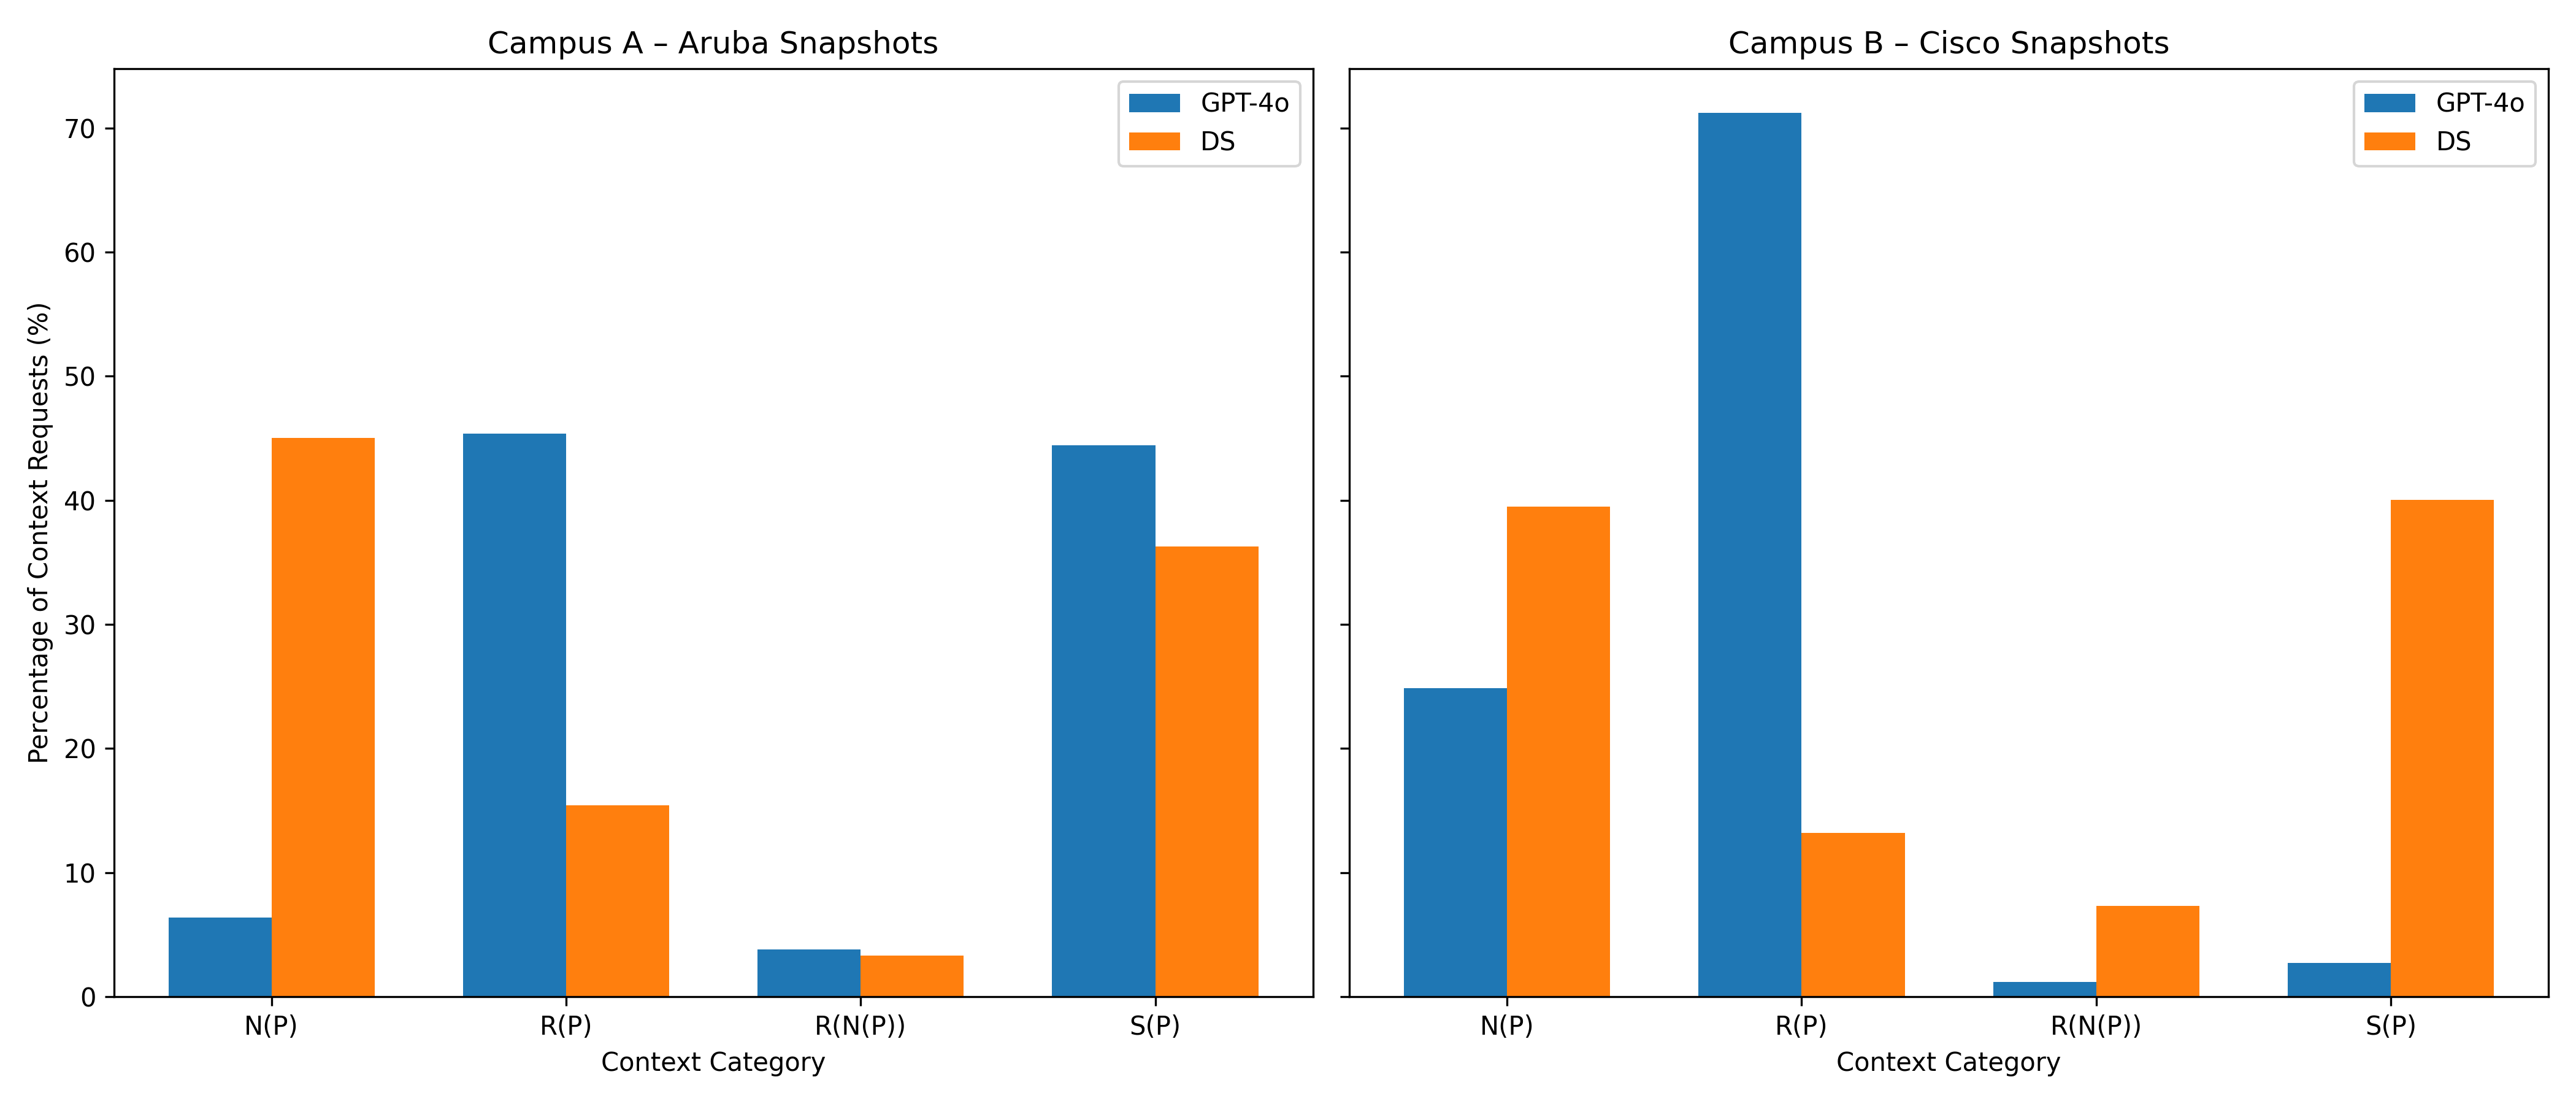
\includegraphics[width=\linewidth]{figs/context_usage_campus_a_b_combined.png}
    \caption{Distribution of context categories requested by GPT-4o and DS.}
    \label{fig:context-usage}
\end{figure}

\paragraph{Non-Targeted Analysis (Campus A):}
In the non-targeted analysis for Campus A snapshots, \sysname{} was able to detect several types of misconfigurations across the provided configuration snapshots, as shown in Table~\ref{tab:real_results}. The detection results are consistent between both implementations of \sysname{} with GPT-4o and DS.
We categorize detected misconfigurations by severity based on their potential impact on network operations: \aaron{This wording creates the impression that we categorized the misconfigs into severity levels by hand, but I think the LLM did the categorization.}
\begin{itemize}
    \item \textit{High Severity}: Misconfigurations in this category pose critical risks to the network and require immediate action \aaron{Should severity levels be defined in the methodology instead of the evaluation?} --- \sysname{} identified invalid subnet mask (\eg, 255.255.253.0) usages that violate binary boundary rules, which could lead to routing issues and network instability.
    \item \textit{Low Severity}: These issues may not immediately disrupt network operations but should be addressed to ensure optimal functionality and avoid potential risks---
    \sysname{} identified many instances of misnamed configurations (\eg, `smnpread' instead of `snmpread' for `snmp\_communities') and inclusion of insecure SSH key exchange (KEX) algorithm (`diffie-hellman-group14-sha1'), which do not break the system but could lead to confusion and maintenance challenges.
    % \item \textit{Low Severity}: These issues present a potential risk but are not critical ---  \sysname{} identified the use of an insecure SSH KEX algorithm (`diffie-hellman-group14-sha1'), which, while outdated, still allows secure communications through stronger algorithms present in the configuration.
    \item \textit{Ambiguous}: These misconfigurations are related to configurations that lead to undefined or nondeterministic behaviors --- \sysname{} found ambiguous rate limit values (`interval' and `burst' set to 0), which can cause unpredictable performance issues due to missing documentation on how these values should be handled, suggesting updates or further specifications in the documentation are needed.
\end{itemize}

Specifically, \sysname{} successfully identified 19 misconfigurations, including two cases of invalid subnet masks, 14 instances of inconsistent policy naming, one insecure SSH KEX algorithm, and two ambiguous rate limit values. Validated with domain experts, we find all misconfiguration cases are either valid or justifiable with a true positive rate (TPR) of 100\% across all targeted misconfigurations.

\paragraph{Non-Targeted Analysis (Campus B):}
In contrast to the genuine misconfigurations identified in Campus A, all configurations flagged in the Campus B snapshot (Table~\ref{tab:grouped_misconfig_analysis}) were subsequently identified by network operators as false positives. Representative cases include:

\begin{itemize}
\item \textit{Duplicate or overlapping DHCP helpers}, which were flagged by both models but were intentionally deployed for redundancy and failover.

\item \textit{Missing VLANs in trunk links} and \textit{Uncoordinated channel-group assignments}, which appeared inconsistent when viewed in isolation but were confirmed to be benign due to compensatory downstream configurations and manual overrides.

\item \textit{Unexpected PIM passive usage}, which aligned with localized multicast policies specific to the campus, albeit undocumented in standard configuration templates.
\end{itemize}

Interestingly, GPT-4o consistently classified all instances as misconfigurations, while DeepSeek-V3 exhibited more conservative behavior—labeling only a subset as problematic (e.g., 4 out of 8 DHCP helper cases, and 0 out of 9 missing VLAN instances). We now proceed to conduct a more detailed analysis of these false positives and inter-model discrepancies.


\aaron{Reviewers may complain that there is no discussion of the true negative or false negative rate. The analysis of known synthetic misconfigurations seems like the best we can do in this regard. Being explicit about this would show that we thought about this limitation of our evaluation---which is also a limitation of of the evaluation of many (all?) other verifiers.}

\subsection{Analysis of False Positives and Model Discrepancies}
\label{subsec:analysis}

To understand how false positives arise within the \sysname{} framework, we conduct a detailed investigation of configuration lines that were incorrectly flagged as misconfigurations by either GPT-4o or DeepSeek, despite being confirmed as correct by human experts. Importantly, these misclassifications are not caused by label noise or inadequate context. \aaron{I would argue these misclassifications are in fact caused by inadequate context. In many cases, \sysname{} could provide the necessary context but the LLM did not request it, which we can see from the differences in context requested by GPT-4o and DS. In other cases, additional context may allow the LLM to detect it--e.g., providing a list of DHCP servers in the network and not simply context from the configurations themselves.} In \sysname{}, the model itself explicitly selects what context it wants to see—including:

\begin{itemize}
    \item $N(P)$: neighboring lines in the configuration file,
    \item $R(P)$: definitions or explanations directly linked to the configuration statement,
    \item $R(N(P))$: definitions referenced by surrounding configuration lines, and
    \item $S(P)$: other configuration lines with a similar structure or syntax elsewhere in the same file.
\end{itemize}
\aaron{Do we need to repeat this list here, because it's already in the methodology section?} \aaron{Also, what about inter-file context?}

Once requested, \sysname{} faithfully provides the exact lines or definitions without transformation or interpretation. This separation ensures that downstream decisions—correct or incorrect—are entirely the result of the model’s own reasoning over the self-curated input context.

\paragraph{Quantitative Comparison.}
GPT-4o falsely flagged all 21 configuration lines in the Campus B dataset as misconfigurations. In contrast, DeepSeek correctly identified 17 of these lines as benign, producing only 4 false positives. This divergence highlights a fundamental difference in inference behavior between the models: GPT-4o is recall-oriented, erring on the side of caution by flagging even subtle or implied inconsistencies. DeepSeek, on the other hand, adopts a more conservative stance, surfacing misconfigurations only when deviations from established patterns are more pronounced or when potential functional impact is apparent. \aaron{This seems like an overly strong conclusion to draw, given the limited set of configurations included in our analysis and the fact that different LLMs request different contexts. For example, if we were to forcibly provide GPT-4o with the additional context requested by DS, would GPT-4o avoid reporting a false positive?}

\paragraph{Context Request Patterns as Diagnostic Signal.}
We analyzed the types of context each model requested to support its predictions. This serves as a window into each model’s internal reasoning strategy:

\begin{itemize}
    \item \textbf{GPT-4o} heavily favored $R(P)$ (requested in 71\% of cases), focusing on keyword-level definitions—such as protocol options, access control lists (ACLs), and helper addresses. It made fewer requests for neighboring lines ($N(P)$) or similar lines ($S(P)$), often assessing a configuration statement in isolation. This explains GPT-4o’s tendency to raise concerns when expected support structures were not explicitly visible in the retrieved definition, even when such structures were defined elsewhere or were optional.

    \item \textbf{DeepSeek} distributed its requests more evenly: 40\% for $N(P)$, 40\% for $S(P)$, only 13\% for $R(P)$, and 7\% for $R(N(P))$. Instead of interpreting a single line in depth, DeepSeek looked at how the current line compared to nearby lines and peer configurations across the file. This behavior led to higher tolerance for configurations that reused common patterns or deviated slightly from canonical forms.
\end{itemize}

\aaron{Do the differences in requested context between the models imply that our design choice of letting the LLMs decide which context to request is actually a bad design choice? I realize we switched to an "ask for the context you need" design to help avoid the issues caused by context overload, but have we swung too far in the opposite direction of not providing enough context? Is it worthwhile to conduct an ablation study that shows what happens if we provide all forms of context to the LLM instead of letting the LLM choose?}

DeepSeek also demonstrated greater efficiency, using fewer tokens per prompt on average (147.9 vs. 180.2 for GPT-4o), while achieving higher prediction accuracy. This suggests that DeepSeek is more effective at extracting signal from minimal but contextually relevant data.

\paragraph{Qualitative Patterns in False Positives.} \aaron{This seems partially redundant with the discussion of the non-targeted campus B results at the end of Section 6.3. Following the restructuring I suggested in my comment at the beginning of the Evaluation section would hopefully address this.}
Three common configuration motifs accounted for the majority of false positives. Below, we contrast the model behaviors on these patterns:

\paragraph{1. \texttt{Shared ip helper-address Across VLANs}}  
Many VLAN interfaces forwarded DHCP requests to the same centralized helper IP. GPT-4o flagged these as potential misconfigurations due to the absence of accompanying ACLs or forwarding rules in the retrieved $R(P)$. \aaron{Can we confirm that this is the issue and reasoning reported by the LLMs? I recall \sysname{} reporting issues with multiple DHCP helper addresses on a single interface, but I don't recall \sysname{} reporting issues with the same DHCP helper address being used on different interfaces. Also, I don't recall anything about ACLs being involved in the LLM's (faulty) reasoning about DHCP server addresses.} However, these rules were defined in other parts of the configuration or not required on that interface. DeepSeek reviewed similar use cases via $S(P)$ and saw consistent repetition of the helper address, correctly judging the setup as intentional.

\paragraph{2. \texttt{VLAN Lists on Trunk Ports with Partial Overlap}}  
Some interfaces allowed a subset of VLANs that were permitted elsewhere in the trunk group. \aaron{Do you mean permitted in other trunk groups? ``Permitted elsewhere'' in the trunk group would imply that the configuration of the different interfaces participating in the trunk, along with the trunk interface itself, were consistent, which I would consider an actual misconfiguration. I'm not even sure you can define allowed VLANs on the individual interfaces participating in a trunk; I think you can only define allowed VLANs on the trunk interface itself.} GPT-4o flagged such cases due to missing VLAN IDs in its $R(P)$ view, \aaron{Having missing VLAN IDs in $R(P)$ implies that \sysname{} didn't extract all $R(P)$ that it should have. Is there a bug in \sysname{}? Is $R(P)$ being truncated?} interpreting them as misalignment. In contrast, DeepSeek leveraged $N(P)$ and $S(P)$ to confirm that partial overlap was common in this deployment and not indicative of configuration drift.

\paragraph{3. \texttt{Presence of Less Common Commands in Valid Contexts}}  
Lines like \texttt{ip pim passive} appeared suspicious to GPT-4o, which interpreted them as incomplete or unsupported, given its limited semantic grounding. \aaron{How do you know GPT-4o has "limited semantic grounding"?} DeepSeek took a more literal view—if the syntax was valid and no contradiction appeared in nearby or similar lines, it labeled them benign.

\paragraph{Implications for Framework and Model Choice.}
These observations highlight a key strength of \sysname{}: the framework strictly limits context to what the model explicitly requests. \aaron{If I recall correctly, DS requested more contexts than GPT-4o, so letting the LLM decide what to request actually seems like a limitation of \sysname{}. As noted above, an ablation study where all forms of context are provided could be a valuable addition.} This ensures that false positives are not a result of hallucinated or poorly stitched context but stem directly from how the model interprets the information it asked for.

By design, \sysname{} decouples \textit{context retrieval} from \textit{context reasoning}. As such, false alarms or overlooked issues can be traced back to model behavior—not to framework artifacts.

The contrasting behaviors of GPT-4o and DeepSeek reflect two ends of a broader tradeoff:

\begin{itemize}
    \item \textbf{GPT-4o (High Recall, Low Precision):}
    \begin{itemize}
        \item Dominated by $R(P)$ requests, focusing on the semantics of the line being analyzed.
        \item Strengths: Good at identifying subtle or undocumented edge cases.
        \item Weaknesses: Flags many benign configurations; lacks robustness in the presence of design variability.
    \end{itemize}

    \item \textbf{DeepSeek (High Precision, Conservative Recall):}
    \begin{itemize}
        \item Emphasizes $N(P)$ and $S(P)$, assessing consistency across peer and nearby configurations.
        \item Strengths: Matches real-world operator expectations and tolerates non-standard but correct setups.
        \item Weaknesses: May miss subtle errors that do not produce visible drift or violate observable patterns.
    \end{itemize}
\end{itemize}

Ultimately, the false positives observed in \sysname{} are not artifacts of random noise—they are deliberate reflections of each model’s interpretive strategy. \sysname{}’s explicit, LLM-driven interface provides a transparent foundation for diagnosing such decisions. The resulting analysis not only informs model selection but also deepens our understanding of how LLMs interpret and reason over structured configuration languages. \aaron{A reviewer might ask: how does a network operator decide which model(s) they should use?}
